\begin{frame}{A Brief Introduction}
   ``Machine learning, neural networks, and artificial intelligence are increasingly being used in orthopaedics for image processing and analysis tasks. These techniques can be used to {\bf automatically analyze medical images} such as X-rays, MRI scans, and CT scans to {\bf extract important diagnostic information} and help with diagnosis and treatment planning. Machine learning algorithms can be trained to {\bf recognize patterns in the images}, and neural networks can be used to process and interpret the data in a more human-like way. These approaches can be used to {\bf identify abnormalities, measure bone density, and classify different types of tissue}, among other tasks. By automating these processes, doctors and other healthcare professionals can {\bf save time and improve the accuracy of their diagnoses}'' \\
\vspace{5mm}
   \hfill - ChatGPT (emphasis mine)
\end{frame}

\begin{frame}{By the end of this presentation, you should be able to \dots}
   \begin{baseitemize}
      \itemR List some ways that deep learning is being used for image processing in orthopaedics
      \itemR Understand some of the basic neural network architectures, and how those fit into different tasks
      \itemR Have a few tips and tricks up your sleeve for getting started with these networks
   \end{baseitemize}
\end{frame}

\begin{frame}{Three Categories of Deep Learning Applications}
   \renewcommand{\arraystretch}{2}
   \begin{center}
            \begin{tabular}{M{0.3\linewidth}|P{0.6\linewidth}}
               \pause Segmentation & Labeling specific pixels of interest in an image \pause \\ \hline
               Classification & Identifying objects in images and determining membership in specific classes \pause \\ \hline
               Detection & Locating regions in images based on presence of specific object
            \end{tabular}
      \end{center}
\end{frame}

\framecard[colorblue]{{\color{white}\hugetext{EXAMPLES}}}

\begin{frame}
   \centering
      \includegraphics[width=\linewidth]{images/histology-title.png}
      \vfill
      \includegraphics[width=0.65\linewidth]{images/histology-images.png}
\end{frame}

\begin{frame}
   \centering
   \includegraphics[width=0.78\linewidth]{images/jtml-title.png}
   \vfill
   \includegraphics[width=0.75\linewidth]{images/jtml-pipeline.png}
   \vfill
   \begin{columns}
      \begin{column}{0.71\linewidth}
         \includegraphics[width=\columnwidth]{images/jtml-nn-image.png}
      \end{column}
      \begin{column}{0.29\linewidth}
         \includegraphics[width=\columnwidth]{images/jtml-registered-implant.png}
      \end{column}
   \end{columns}
\end{frame}

\begin{frame}{Classification of Equine Stifle Pathology}
   \centering
   \includegraphics[width=0.85\linewidth]{images/stifle-pathologies.png}
\end{frame}

\begin{frame}
   \centering
   \includegraphics[width=0.7\linewidth]{images/tka-classification-title.png}
   \vfill
   \includegraphics[width=0.85\linewidth]{images/tka-classification.png}
   \vfill
   \tiny{Karnuta et al., Journal of Arthroplasty, 2021\\ doi:10.1016/j.arth.2020.10.021}
\end{frame}

\begin{frame}
   \centering
         \includegraphics[width=0.65\columnwidth]{images/hrnet-title.png}
   \vfill
   \includegraphics[width=\linewidth]{images/hrnet-human-pose.png}
   \vfill
   \tiny{Wang et al, Computer Vision and Image Understanding, 2021 \\ doi: 10.1016/j.cviu.2021.103225}
\end{frame}

\framecard[colorblue]{\color{white}\hugetext{WHAT IS DEEP LEARNING FOR IMAGE PROCESSING?}}

\begin{frame}{A Basic Definition}
   \begin{columns}
      \centering
      \begin{column}{0.4\linewidth}
         \begin{baseitemize}
            \itemR Subset of machine learning using neural networks to imitate the visual system in the brain
            \vspace{0.45in}
            \itemR A set of algorithms that learn programs from data
         \end{baseitemize}
      \end{column}
      \begin{column}{0.6\linewidth}
         \centering
            \includegraphics[width=0.8\columnwidth]{images/visual-nn.png}\\
            \tiny{Cox and Dean, Neural Networks and Neuroscience-Inspired Computer Vision, 2014}
      \end{column}
   \end{columns}
\end{frame}


\begin{frame}{The Architecture of a Neural Network}
   \centering
   \renewcommand{\arraystretch}{1.5}
   \begin{tabular}{c|c}
      \Large{Building Block} & \Large{Neural Network} \\ \hline \pause
      {\includegraphics[width=1in, valign=m,margin = 1pt]{images/neuron.png} $\phi(\sum_{i=1}^n a_i w_i)$} & \includegraphics[width=1.25in, valign=m, margin = 1pt]{images/fcn.png} \\ \hline \pause 
      \includegraphics[width = 1.3in, valign=m, margin = 1pt]{images/2d-convolution.png} & \includegraphics[width=1.85in, valign=m, margin = 1pt]{images/u-net.png}
   \end{tabular}
\end{frame}

\begin{frame}{The Power of Convolutional Neural Networks}
   \centering
   \includegraphics[width=0.6\linewidth]{images/conv-layers.png}\\
   \tiny{Shulz and Behnke, Deep Learning: Layer-Wise Learning of Feature Hierarchies, 2012}
\end{frame}

\framecard[colorblue]{{\color{white}\hugetext{ARCHITECTURE MODIFICATIONS}}}

\begin{frame}{Classification}
   \centering
   \includegraphics[width=0.8\linewidth]{images/classification.png}
\end{frame}

\begin{frame}{Segmentation}
   \centering
   \includegraphics[width=0.8\linewidth]{images/segmentation.png}
\end{frame}

\framecard[colororange]{{\color{white}\hugetext{TIPS AND TRICKS}}}

\begin{frame}{You Can't Outrun A Lack of Data}
   \centering
   \includegraphics[width=0.25\linewidth]{images/data_trap.png}
   \vfill \tiny{https://xkcd.com/2582/}
   \vfill
   \includegraphics[width=0.7\linewidth]{images/augmentations.jpg}
   \vfill \tiny{https://albumentations.ai/}

\end{frame}

\begin{frame}{Minimal Necessary Force}
   \centering
   \includegraphics[width=0.45\linewidth]{images/xkcd-ml.png}
   \vfill \tiny{https://xkcd.com/1838/}
\end{frame}

\begin{frame}
   \frametitle{Utilizing Historic Methods}
   \centering
   \begin{columns}
      \begin{column}{0.25\linewidth}
         \centering
         \includegraphics[width=\columnwidth]{images/tasks.png}
         \vfill \tiny{https://xkcd.com/1425/}
      \end{column}
      \begin{column}{0.75\linewidth}
         \centering
         \includegraphics[width=0.85\columnwidth]{images/perspective-projection.png}
      \end{column}
   \end{columns}
\end{frame}

\framecard[colororange]{{\color{white} \hugetext{GETTING STARTED}}}

\begin{frame}
   \frametitle{MONAI}
   \centering
   \includegraphics[width=0.68\linewidth]{images/monai.png}
   \vfill \tiny{https://monai.io}

\end{frame}

\begin{frame}{Background Information}
   \begin{baseitemize}
      \itemR CS231n: Deep Learning for Computer Vision, Stanford University (http://cs231n.stanford.edu/, lectures on YouTube)
      \itemR Andrew Ng Coursera Courses
      \begin{baseitemize}
         \itemR Machine Learning Specialization
         \itemR Deep Learning Specialization
      \end{baseitemize}
   \end{baseitemize}
\end{frame}

\framecard[colororange]{{\color{white} \hugetext{CASE STUDY}}}

\begin{frame}{The Problem}
   \begin{baseitemize}
      \itemR 20\% of patients recieving TKA are dissatisfied
      \itemR Clinicians don't have the ability to routinely quantify joint kinematics
      \begin{baseitemize}
         \itemR They must rely on manual examination and static imaging
         \itemR Historic methods of measuring joint kinematics require are too time consuming for routine clinical use
      \end{baseitemize}
   \end{baseitemize}
   \vfill \pause Question: Can we automate the process of measuring joint kinematics in order to make these measurements clinically feasible?
\end{frame}

\begin{frame}{Joint Track Machine Learning: Data}
   \centering
   \begin{columns}
      \begin{column}{0.4\linewidth}
         \includegraphics[width=\columnwidth]{images/jtml-data.png}
      \end{column}
      \begin{column}{0.6\linewidth}
         \includegraphics[width=\columnwidth]{images/jtml-segmentation.png}
      \end{column}
   \end{columns}
\end{frame}

\begin{frame}{Joint Track Machine Learning: Historic Methods and Minimal Necessary Force}
   \centering
   \includegraphics[width=0.7\linewidth]{images/jtml-pipeline.png}
   \begin{columns}
      \begin{column}{0.55\linewidth}
         \centering
         \includegraphics[width=\columnwidth]{images/jtml-nfd.png} 
         \vfill 
         \scalebox{0.35}{Wallace and Mitchell, Analysis of three-dimensional movement using Fourier descriptors, 1980} \\
         \scalebox{0.35}{Wallace and Wintz, An efficient three-dimensional aircraft recognition algorithm using normalized fourier descriptors, 1980} \\
         \scalebox{0.35}{Banks and Hodge, Accurate measurement of three-dimensional knee replacement kinematics using single-plane fluoroscopy, 1996} \\
      \end{column}
      \begin{column}{0.45\linewidth}
         \centering
         \includegraphics[width=0.7\columnwidth]{images/jtml-registered-implant.png}
         \vfill
         \scalebox{0.35}{Jones et al, Lipschitzian Optimization without the Lipschitz Constant, 1993}
      \end{column}
   \end{columns}
\end{frame}

\framecard[colororange]{{\color{white} \hugetext{THANK YOU\\ajensen123@ufl.edu}}}
% \begin{fullpageitemize}
%  \item {\montserratfont This is Montserrat}
%  \item {\notosansfont This is Noto Sans}
%  \item {\latolightfont This is Lato (light)}
%  \item {\inconsolatafont This is inconsolata}
%  \item \textsc{This is Alegreya Sans small caps}
% \end{fullpageitemize}
%\end{frame}


%\begin{frame}{Color Palette}
% \begin{center}
% \crule[colordgray] \crule[colorhgray] \crule[colorblue] \crule[colorgreen] \crule[colororange]
% \end{center}
%\end{frame}

%\framecard[colorgreen]{{\color{white}\hugetext{BIG BOLD TEXT}}}

%\framepic[0.8]{images/skeleton}{
% \begin{textblock}{7}(7,2.5)
%    {\color{colorblue}\hugetext{\textbf{RUN!}}}
% \end{textblock}
%}